% Font options: 10pm, 11pt, 12pt
% Align headings left instead of center: nocenter
\documentclass[11pt, nocenter, letter paper, oneside]{book}

%\includeonly{text/introduction} % Use this for editing just one section

\usepackage{indentfirst, amsmath, setspace, amssymb, amsthm}

\usepackage{lipsum} % For placeholder text. Delete this.

\usepackage{natbib}
\bibliographystyle{apsr2006}

\usepackage{graphicx}
\usepackage{hyperref}

%%%%%% FONT OPTIONS %%%%%%
%\usepackage{mathptmx} % Times New Roman
%\usepackage{mathpazo} % Palatino
%\usepackage[osf]{mathpazo} % Palatino with old-style numerals
%%%%%%%%%%%%%%%%%%%%%%%%%%

\usepackage{graphicx} 
\usepackage{pgf,tikz}
\usepackage{pgfplots}
\usetikzlibrary{arrows,shapes}
\usetikzlibrary{decorations}

%\usepackage{pdflscape}
\usepackage{mathtools}
\usepackage{upgreek} 
\usepackage{xfrac}
\usepackage{epstopdf}
\usepackage{color}
\usepackage{array}
\usepackage{booktabs}
\usepackage{longtable} 
\usepackage{verbatim}

\setcounter{tocdepth}{1} % Include Subsections (but not subsubsections) in the TOC
\usepackage[T1]{fontenc}

\usepackage{pdfpages} % For including the Dissertation Acceptance Certificate

%%%%%% CHAPTER TITLE OPTIONS %%%%%%
\usepackage{titlesec}
\definecolor{gray75}{gray}{0.75}
\newcommand{\hsp}{\hspace{20pt}}
\titleformat{\chapter}[hang]{\singlespace\LARGE\bfseries}{\thechapter\hsp\textcolor{gray75}{|}\hsp}{0pt}{\LARGE\bfseries} % Title format for numbered chapters
\titleformat{name=\chapter,numberless}[hang]{\singlespace\LARGE\bfseries}{\textcolor{gray75}{|}\hsp}{0pt}{\LARGE\bfseries} % Title format for unnumbered chapters (intro, contents, bib, etc.)
%%%%%%%%%%%%%%%%%%%%%%%%%%%%%%%%%%%

\DeclareGraphicsRule{.tif}{png}{.png}{`convert #1 `dirname #1`/`basename #1 .tif`.png}

% Theorem environments
\theoremstyle{plain}
\newtheorem{prop}{Proposition}
\newtheorem{cor}{Corollary}
\newtheorem{thm}{Theorem}

% Margin must be at least 1in on all sides.
\usepackage[left=1.25in, right=1.25in, top=1.25in, bottom=1.25in, footskip=.25in]{geometry}
% This makes footnotes appear to be single spaced within each entry, but double spaced between entries.
\setlength{\footnotesep}{16pt}

\pagestyle{plain}

\begin{document}

%%%%%%%%%%%%%%%%%%%%%%%%%%%%%%%%%%%%%%%%%%%%%%%%%%%%%%%%%%%%%%%%%%%%%%
% Include these lines after the defense when you 
% get a scan of the dissertation acceptance certificate.
% This makes the DAC the first page, and then adds a blank page
%
%	\includepdf[pages={1}]{dissertation_acceptance_certificate.pdf}
%	\newpage
%	\thispagestyle{empty}
%	\mbox{}
%
%%%%%%%%%%%%%%%%%%%%%%%%%%%%%%%%%%%%%%%%%%%%%%%%%%%%%%%%%%%%%%%%%%%%%%

% Frontmatter with roman numerals
\frontmatter
\thispagestyle{empty}
\begin{center}
\vspace*{2.0 in}
{\LARGE \bf A Most Important Study}\\

\vspace{4em}  
A dissertation presented
\\~\\
by
\\~\\
{\large Author Full Name}
\\~\\
to
\\~\\
The Department of Government
\\~\\
in partial fulfillment of the requirements \\
for the degree of \\
Doctor of Philosophy\\
in the subject of\\
Political Science
\\~\\
Harvard University\\
Cambridge, Massachusetts
\\~\\
Month 2014
\end{center}

\thispagestyle{empty}

\vspace*{3in}
\indent \copyright \emph{2014 --- Author Full Name}
\\~\\
\indent All rights reserved.

\phantomsection % Needed to make the ToC links work properly
% Abstract
\noindent Dissertation Advisor: Advisor Name \hfill Author Full Name
\addcontentsline{toc}{chapter}{Abstract}

\doublespacing

\begin{center}
\vspace{0.5 in} \LARGE{\bf A Most Important Study}

\vspace{0.25in}
\large{\textbf{Abstract}}
\end{center}

This dissertation studies the most important question in political science. \lipsum[1-2]


\singlespacing
\tableofcontents
%\listoffigures
%\listoftables

\doublespacing
\phantomsection % Needed to make the ToC links work properly
% Acknowledgments
\chapter*{Acknowledgments}
\addcontentsline{toc}{chapter}{Acknowledgments}

So many people to thank. List them here. Say something nice.
\mainmatter

\phantomsection % Needed to make the ToC links work properly
\chapter*{Introduction}
\addcontentsline{toc}{chapter}{Introduction}

If you wrote three papers, write a few pages that attempts to connect them here. If you wrote a book, you will probably delete this section and start with Chapter 1.

\lipsum[1-4]
	
	
	
\chapter{The First Paper/Chapter}

\section{Introduction}

We begin with the most important question in political science. \lipsum[1]

\section{Literature}

The literature on this question begins with  \citet{tocqueville1838} and \citet{wilson1885}. There is also some more literature \citep{downs1957,baron1989,cox1993,krehbiel1998}. \lipsum[2]

\section{Some Results}

\lipsum[3] 

\begin{table}[htbp]
\caption{Captions for Tables Go \textbf{ABOVE} the Table}
\label{tab:fjc_summary}
\begin{center}
\begin{tabular}{llrrrrrrr}
\toprule
& First & Total & Appts. & Appts. & Avg. & Original & Current & Currently\\
Court & Year & Appts. & Per Year & Per Pres. & Tenure & Seats & Seats & Serving\\
\midrule
USSC & 1789 & 117 & 0.53 & 2.67 & 16.06 & 6 & 9 & 9 \\ 
USCA & 1891 & 729 & 6.18 & 26.42 & 13.87 & 18 & 179 & 164 \\ 
USDC & 1789 & 2826 & 12.85 & 61.70 & 14.56 & 13 & 673 & 597 \\ 
\bottomrule
\end{tabular}
\end{center}
\end{table} 

\lipsum[4]

\begin{figure}[htbp]
   \centering
   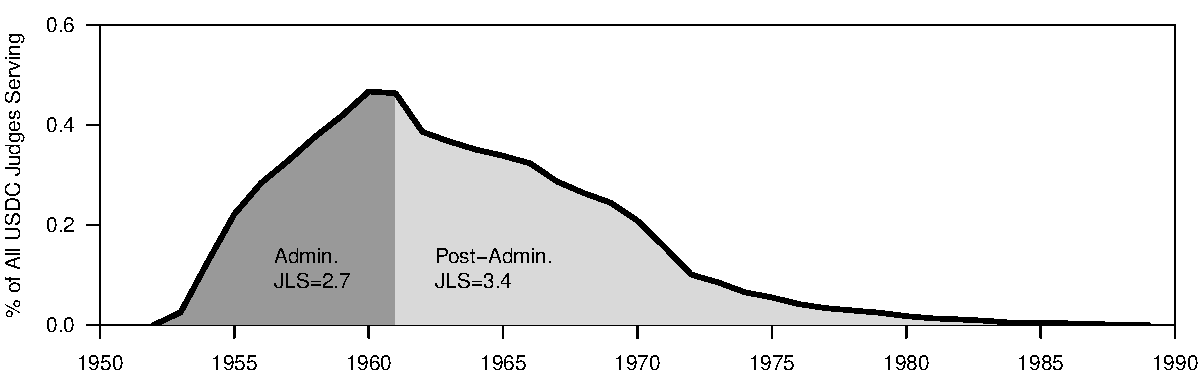
\includegraphics[width=\textwidth]{figures/example_figure.pdf}
   
\caption{Captions for Figures Go \textbf{BELOW} the Figure}
\end{figure}

\lipsum[5]

\section{Conclusion}
\lipsum[6-7] 
\chapter{The Second Paper/Chapter}

\section{Introduction}
\lipsum[1-4]

\section{Conclusion}
\lipsum[5-8]
\chapter{The Third Paper/Chapter}

\section{Introduction}
\lipsum[1-4]

\section{Conclusion}
\lipsum[5-8]

\appendix

\chapter{Appendix to Chapter 1: Data Collection}\label{sec:appendix1}

\lipsum[1-2] % Replace this with text
\chapter{Appendix to Chapter 1: Robustness Checks}\label{sec:app2}

\lipsum[1-2] % Replace this with text
\chapter{Appendix to Chapter 2: Model Extensions}\label{sec:app3}

\lipsum[1-2] % Replace this with text

\chapter{Appendix to Chapter 3: Even More Stuff}

\lipsum[1-2] % Replace this with text


\backmatter

\singlespacing
\phantomsection % Needed to make the ToC links work properly
\addcontentsline{toc}{chapter}{Bibliography}
\bibliography{dissertation}

\end{document}
